\chapter{Background and Related Work}
\thispagestyle{main} % Needed for Footer and Header on Chapterpage

The section \textit{Background} introduces the tools and technologies used in the Bazo Blockchain. In the section \textit{Related Work} the theses of other students who worked on the Bazo Blockchain and some independent projects are described.

\section{Background}
\subsection{Blockchain}
A blockchain is a distributed database. It consists of blocks of data chained together by hash functions. The data inside these blocks are transactions. In order to make the transactions non-repudiable digital signatures are used. The transactions are validated by a miner. The miner validates the signatures and checks if the assets transmitted by the transaction, usually tokens or coins representing a real monetary value, actually exists on the account of the other person. Since the Bazo Blockchain is account based, it also updates the balance of the account according to the transmitted value. Previous theses in the context of Bazo dive deeper into cryptocurrencies and blockchains. \cite{ba_miner} \cite{ba_client} 

\subsection{Smart Contracts}
A smart contract is basically an agreement or contract written in computer code, saved in a transaction and therefore distributed over the whole network. The smart contract can then be called by another transaction and is executed by a VM which is part of the miner.

\subsection{Transactions}
In the context of data base management systems a transaction is a unit of work performed within the system. \cite{dbtransaction} This definition is also applicable for blockchains. As later explained there are multiple transaction types and only some are used to send coins. Others are used mostly to change the system state or create a new account.

\subsection{Virtual Machine}
A virtual machine is an abstraction layer. A VM abstracts a program or even a whole operating system from the hardware it is actually run on to make it portable.

\section{Related Work}
At the time of writing the thesis, the \href{https://github.com/bazo-blockchain}{Bazo Blockchain Github organization} contains the software systems as described in Figure \ref{systemcontextdiagram}. There are also some smaller tools which are not further described. Figure \ref{systemcontextdiagram} shows the Bazo Blockchain and its most important software systems.  It also describes how the systems interact with each other and with the out world. It shows multiple miner instances to represent the blockchain and to describe how the miners interact with eachother.

\begin{figure}[H]
	\begin{center}
	\includegraphics[width=0.83\textwidth]{./images/BAZO_System_Context}
	\caption{Bazo Blockchain system context diagram}
	\label{systemcontextdiagram}
	\end{center}
\end{figure}

\begin{tabular}[t]{ p{3cm} p{12.5cm}}
\textbf{Miner} &
The miner is at the heart of the blockchain. It validates transactions, keeps the ledger up to date, executes smart contracts via the VM and broadcasts new transactions or blocks to other miners. \\ \\
 
\raggedright
\textbf{Wallet} &
The wallet allows user to operate on the blockchain. It also stores the public/private key pair. \cite{ba_wallet} \\ \\
 
\textbf{Client} &
The client is used to communicate with the miner by creating and sending new transactions. \\ \\

\raggedright
\textbf{Block Explorer} & 
The block explorer is used to view transactions. It basically visualizes the blockchain. \\ \\

\raggedright
\textbf{Miscellaneous} & 
There are also some smaller tools, like keypairgen but they are not further discussed here. The organization on Github is accessible under the following link: \href{https://github.com/bazo-blockchain}{https://github.com/bazo-blockchain}. \\ \\
\end{tabular}

\subsection{How Bazo Works - an Overview}
In Figure \ref{systemcontainerdiagram} one of the miners is expanded, which makes it possible to see its packages and their relationships with other components. 

As shown in Figure \ref{systemcontainerdiagram} the transactions sent by the user over the Web API are received and processed by the \Gls{p2p} package. If it receives a new transaction it will add it to the unprocessed transaction pool via the storage package. 

The miner will continuously fetch transactions from the unprocessed transactions pool, verify their signature and their validity, add the transaction hash to the current block and save the transaction in the processed transaction pool. If the transaction calls a contract, the miner will call the VM and it will execute the called contract function. After that, the miner will change its state according to the results of the VM.

\begin{figure}[H]
	\begin{center}
	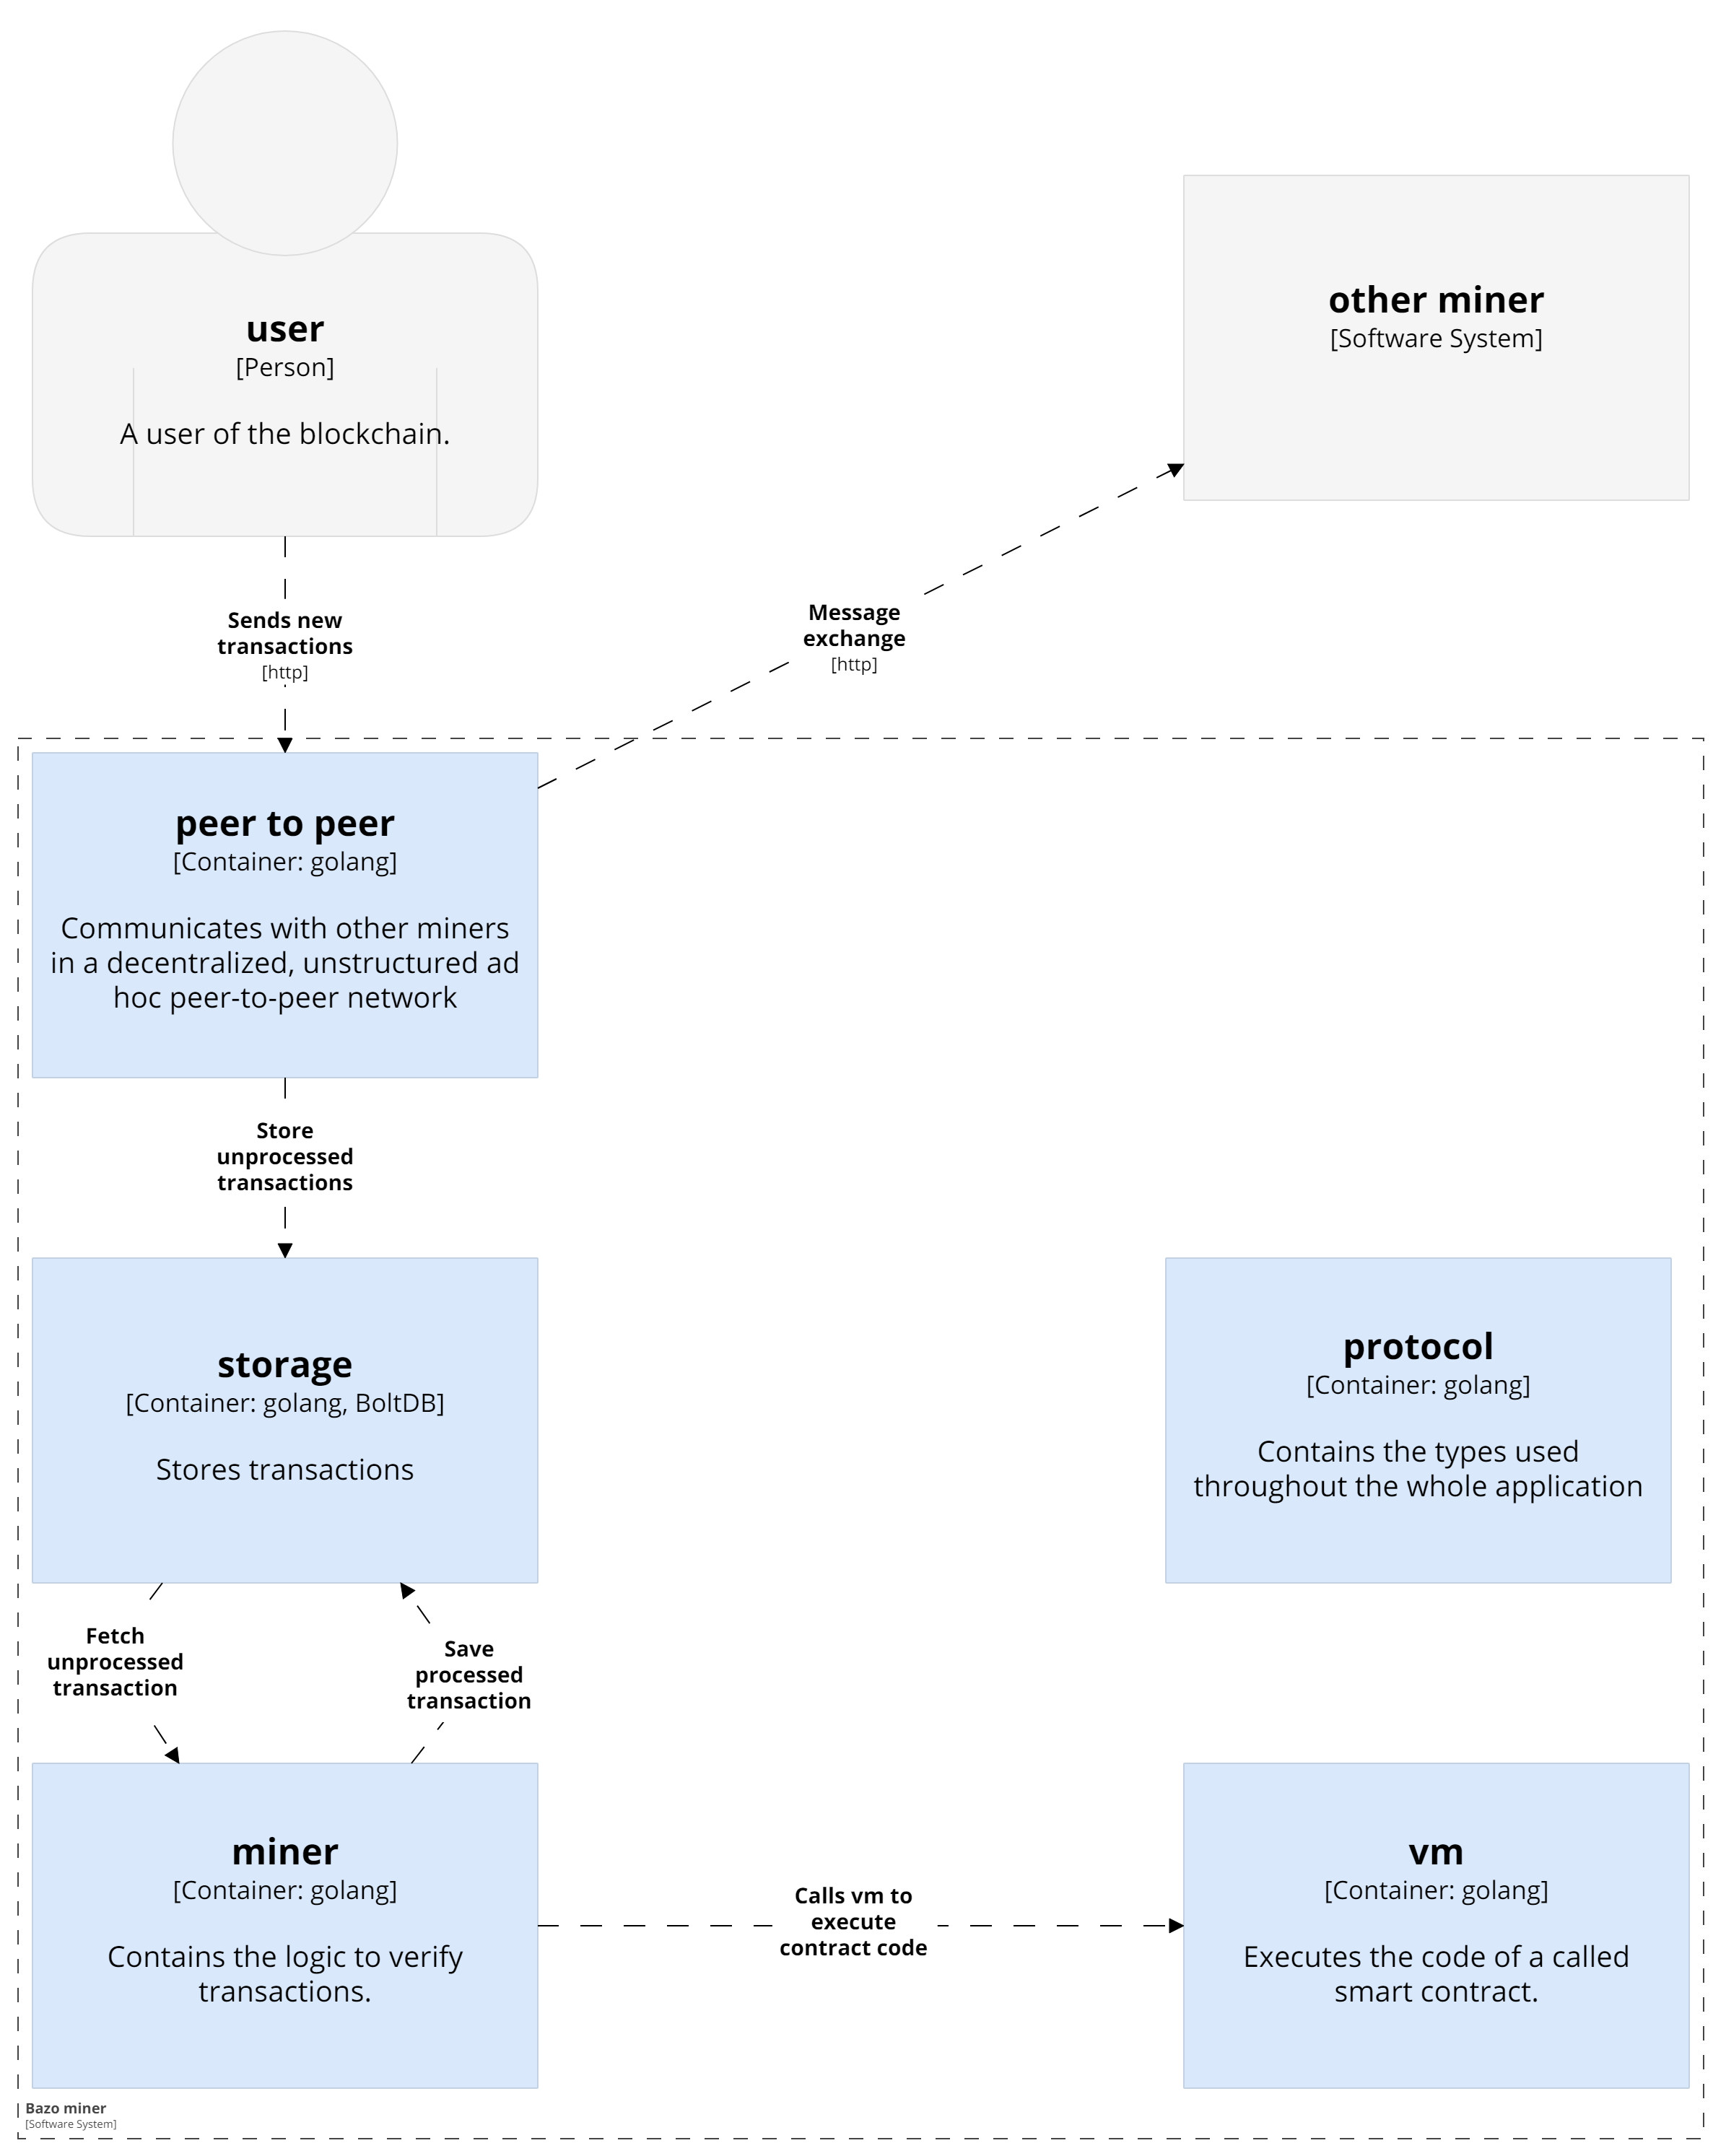
\includegraphics[width=0.8\textwidth]{./images/BAZO_Container}
	\caption{Bazo Blockchain container diagram}
	\label{systemcontainerdiagram}
	\end{center}
\end{figure}
\pagebreak

\subsection{Previous work}
As the Bazo Blockchain was started in 2017 there have been several theses. Within these theses different aspects of the blockchain have been implemented. 

\begin{description}
	\item [Bazo – A Cryptocurrency from Scratch \cite{ba_miner}] was written by Livio Sgier. He implemented the miner during this work. He partitioned the software into the P2P, storage, miner and protocol package.
	\item [A Progressive Web App (PWA)-based Mobile Wallet for Bazo \cite{ba_wallet}] was written by Jan von der Assen. His work was a proof of concept for a portable wallet which allows for mobile payments in a sandbox environment. In Figure \ref{systemcontextdiagram} the result of his work is represented as the wallet software system.
	\item [A Blockchain Explorer for Bazo \cite{ba_explorer}] was written by Luc Boillat. The Bazo Blockchain Explorer allows users of the blockchain to inspect blockchain data through a graphical user interface, requiring no installation to use, since the application is available on the internet as a web app. \cite{ba_explorer}
	\item [Proof of Stake for Bazo \cite{ba_pos}] was written by Simon Bachmann. Simon Bachmann studied multiple algorithms and implementations for PoS and chose the best for the later implementation of PoS which was also part of the work.
	\item [Design and Prototypical Implementation of a Mobile Light Client for the Bazo Blockchain \cite{ba_client}] was written by Marc-Alain Chételat. The blocks of the Bazo Blockchain only contain the transaction headers but stores the transactions separately. During his work he implemented a light client which contains only the transaction headers and their hashes but not the actual transactions. This allows a client to also run on mobile devices. He also 	implemented a multi-signature mechanism which allows to verify transactions within three seconds.  To do this a Bazo signature server is used to check if the accounts balance is high enough to send the transaction. If it does, the transaction is signed and therefore verified. 
\end{description}

\subsection{Similar existent projects}
Since the code of NEO and Ethereum is on Github and open source, their implementation has been studied and sometimes been implemented analogously. 

\begin{tabular}[t]{ p{3cm} p{12.5cm}}
\textbf{NEO} &
NEO is a blockchain project \flqq that utilizes blockchain technology and digital identity to digitize assets, to automate the management of digital assets using smart contracts, and to realize a smart economy with a distributed network.\frqq \cite{neovseth} NEO utilizes a consensus mechanism called the Delegated Byzantine Fault Tolerance. NEO is implemented in C\#. \cite{neo_whitepaper}
\end{tabular}

\begin{tabular}[t]{ p{3cm} p{12.5cm}}
\textbf{Ethereum} & 
The goal of Ethereum is to create a platform for the development of decentralized apps in order to create a \flqq more globally accessible, more free, and more trustworthy Internet, an internet 3.0\frqq. \cite{neovseth} There are several implementations of the client such as go-ethereum (written in Go), cpp-ethereum (written in C++) and others. Ethereum's consensus mechanism is Proof of Work but  a Proof of Stake algorithm is already being developed and likely to go live in 2018. \\ \\
\end{tabular}

\begin{tabular}[t]{ p{3cm} p{12.5cm}}
\raggedright
\textbf{What are the differences to Bazo} & 
Both, Ethereum and NEO are public, permission-less smart contract platforms. At the time of writing, the Bazo Blockchain is a permissioned blockchain because of the initial requirements from the financial services provider. As for now, the Bazo Blockchain is just a research project. The goal is to become a public, permission-less platform for decentralized applications. To reach this goal and be able to create and maintain a competitive blockchain, a dedicated team would be needed. \\ \\
\end{tabular}